\documentclass[a4paper,10pt]{article}
\usepackage[utf8]{inputenc}
\usepackage{graphicx}

%opening
\title{Transferring $^3$He to Hifrost Tank}
\author{Ryan Duve}

\begin{document}

\maketitle

\begin{abstract}

\fbox{\parbox{.75\textwidth}{Only workers highly familiar with the technical aspects of Hifrost are authorized to perform this procedure.
}}
\vspace{.5cm}


We will transfer $\sim$40 L $^3$He gas (\textbf{hereafter, He gas}) from pressurized bottles to our 114 L storage tank, T2.  Given the price, scarcity, and central importance of He gas to Hifrost operation, a procedure has been drafted to verify everything goes smoothly during the transfer and will be practiced on a test tank of $^4$He gas.

This document assumes prior knowledge of the Hifrost pumping system and vacuum systems and components in general.  Please consult the Hifrost manual for context of this procedure and definitions/explanations of the system.
\end{abstract}

\section{Prep}
The relevant section of the He gas system is shown in Figure \ref{a}.\begin{figure}[htbp!]
 \centering
 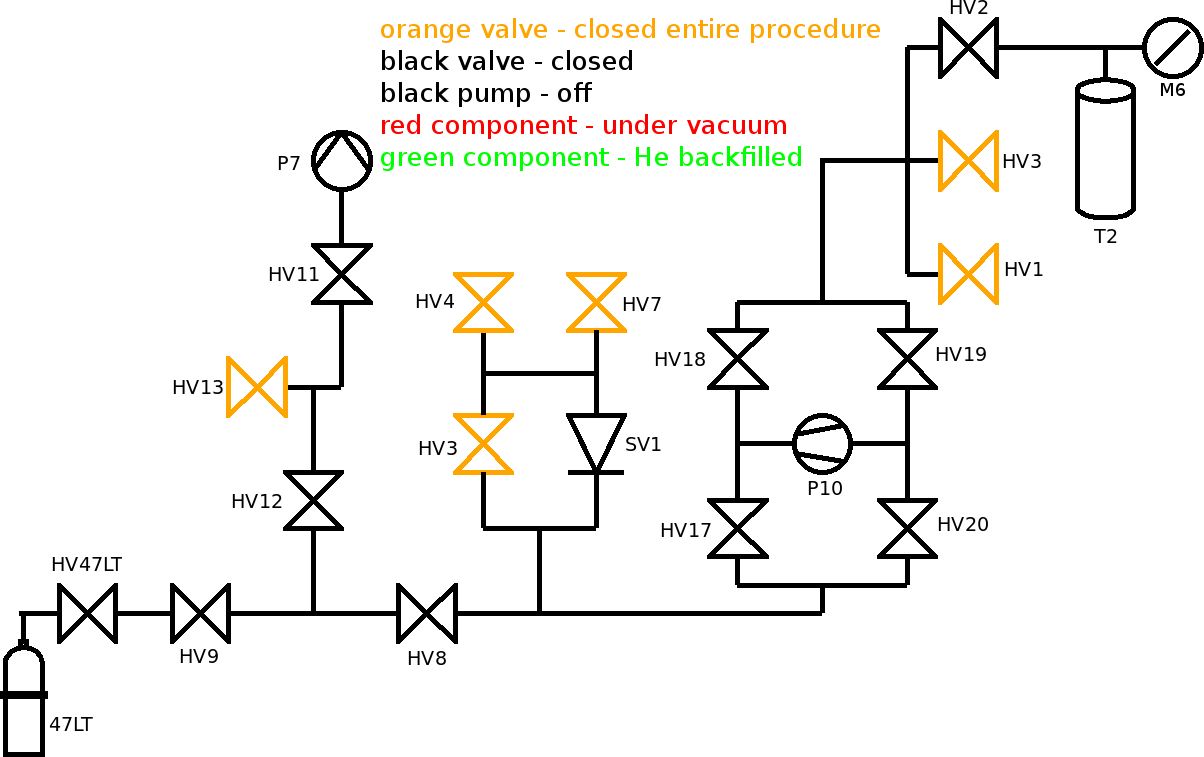
\includegraphics[width=\textwidth]{./he-3-transfer-02-closed-valves.png}
 % he-3-transfer-01-starting.png: 0x0 pixel, 0dpi, 0.00x0.00 cm, bb=
 \caption{The system.}
 \label{a}
\end{figure}

The pressurized bottle 47LT is a 47 L tank that was backfilled to about an atmosphere with $^4$He gas and used as practice for the real transfer.  A regulator will take the place of HV47LT and the bottle replaces 47LT.

\section{Transfer}
\begin{enumerate}
 \item Hook up the system as shown in Figure \ref{a}.  Make sure all orange valves are closed and are not touched until the end of the transfer.  Together they bound the volume the He gas may take up.
 \item Figure \ref{b}: start P7 and evacuate the system via the following path: P7, HV11, HV12, HV8, HV17-20, HV2, T2, and verify the vacuum in T2 with M6.  Also, open HV9 to pull vacuum up to the valve on the pressurized cylinder.
 \item Figure \ref{c}: close valves HV11, HV17 and HV18.  Turn off P7.  There should be a path for He gas to flow from the pressurized cylinder to T2 without any exit to atmosphere.
 \item Figure \ref{d}: slowly open HV47LT, the valve(s) on top of the pressurized cylinder, and watch the pressure M6 rise until it equilibrates with the pressure on the cylinder.  Then open HV47LT all the way.
 \item Figure \ref{e}: close valves HV19 and HV20 and open valve HV18, then turn on P10.
 \item Figure \ref{f}: slow open HV20 and pump He gas out of 47LT and the rest of the pump system into T2.
 \item Figure \ref{g}: when T2 stops rising and the pressure gauge on the pressurized cylinder reads a low vacuum, close HV20, turn off P10, then close HV18 and HV2.
\end{enumerate}

\begin{figure}[htbp!]
 \centering
 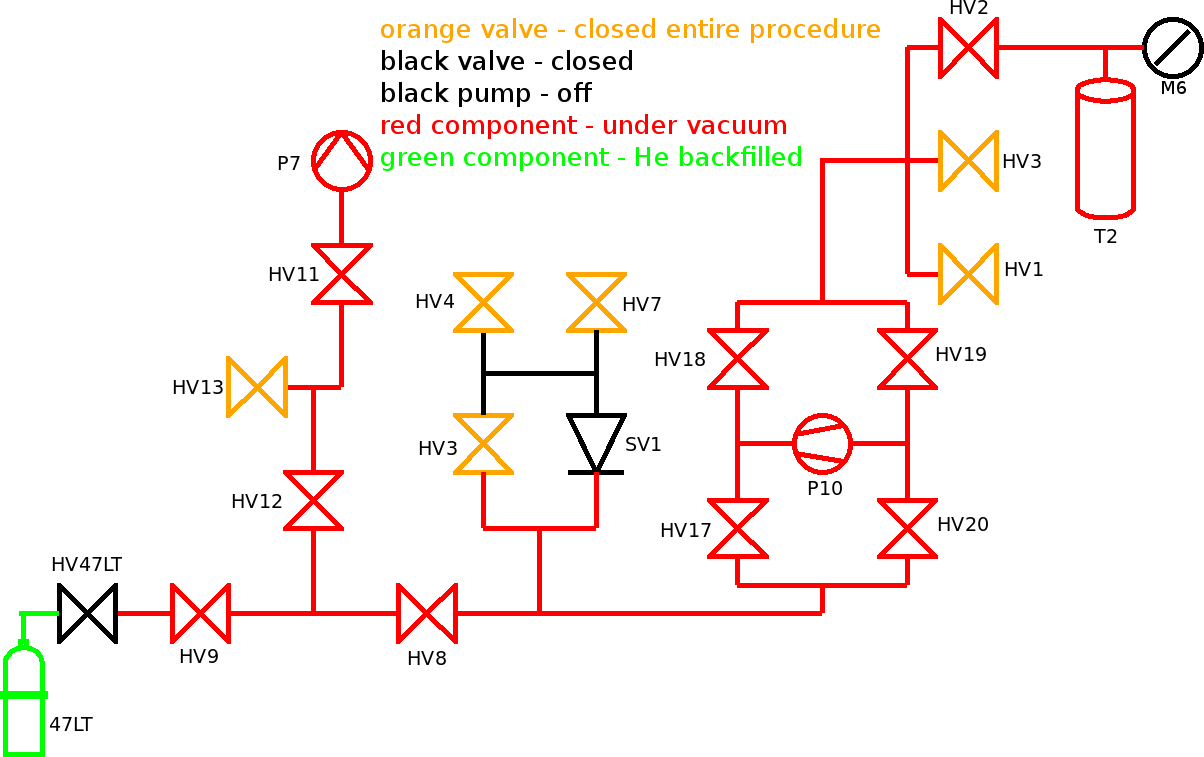
\includegraphics[width=\textwidth]{./he-3-transfer-04-evac-system-with-p7.png}
 % he-3-transfer-04-evac-system-with-p7.png: 0x0 pixel, 0dpi, 0.00x0.00 cm, bb=
 \caption{Evacuate system with P7.}
 \label{b}
\end{figure}
\begin{figure}[htbp!]
 \centering
 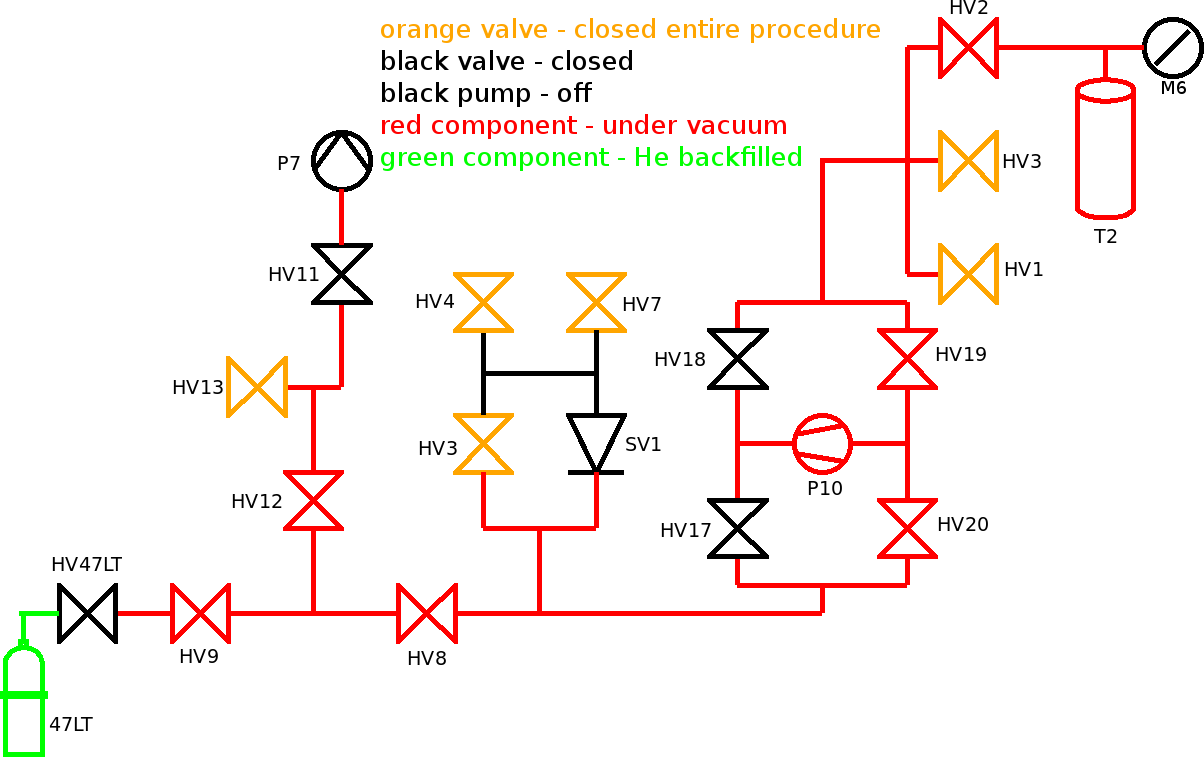
\includegraphics[width=\textwidth]{./he-3-transfer-05-kill-p7.png}
 % he-3-transfer-05-kill-p7.png: 0x0 pixel, 0dpi, 0.00x0.00 cm, bb=
 \caption{Isolate and turn off P7, then close two recovery manifold valves.}
 \label{c}
\end{figure}
\begin{figure}[htbp!]
 \centering
 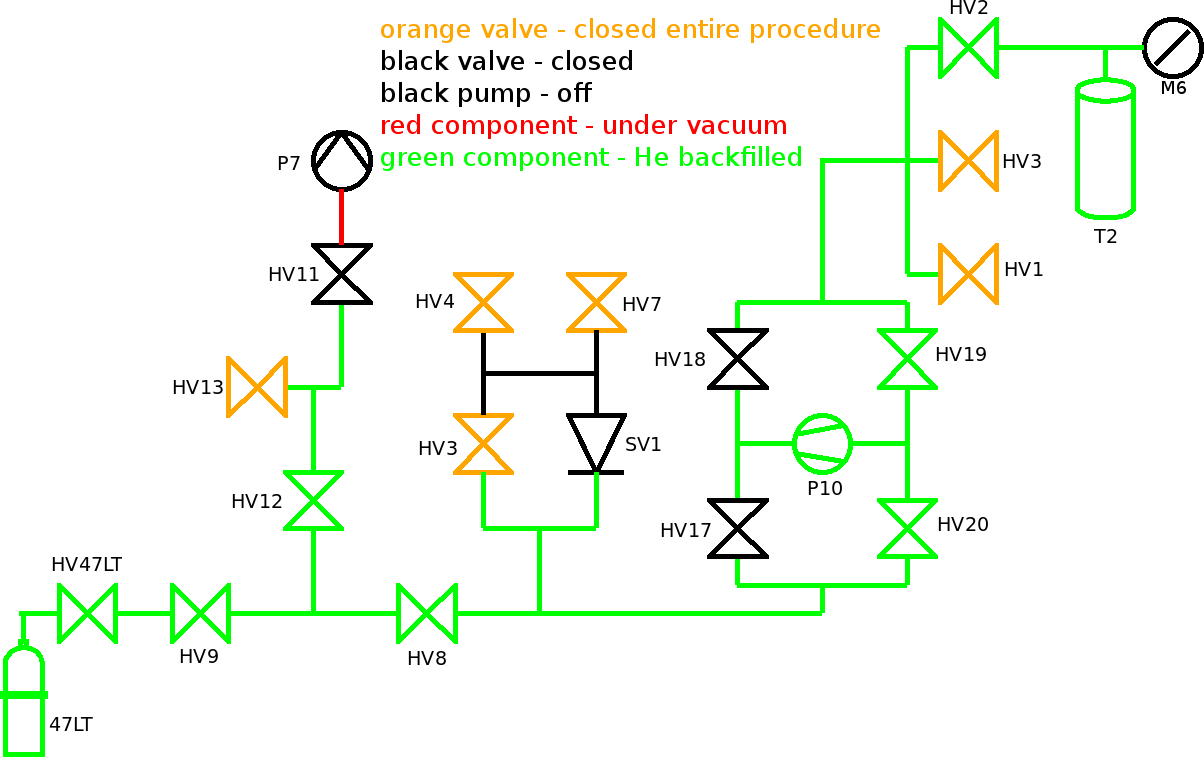
\includegraphics[width=\textwidth]{./he-3-transfer-06-open-hv47lt.png}
 % he-3-transfer-06-open-hv47lt.png: 0x0 pixel, 0dpi, 0.00x0.00 cm, bb=
 \caption{Open the pressurized cylinder and allow the gas to flow into T2.}
 \label{d}
\end{figure}
\begin{figure}[htbp!]
 \centering
 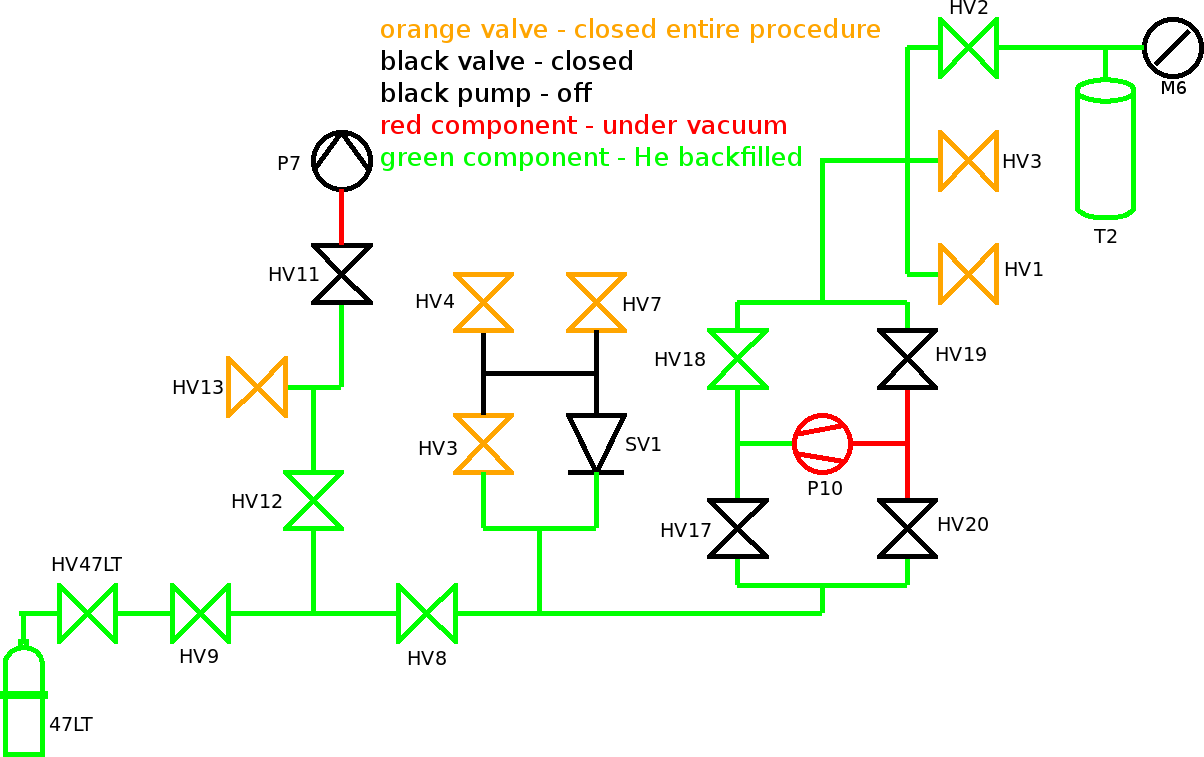
\includegraphics[width=\textwidth]{./he-3-transfer-07-turn-on-p10.png}
 % he-3-transfer-07-turn-on-p10.png: 0x0 pixel, 0dpi, 0.00x0.00 cm, bb=
 \caption{Open/close appropriate recovery valves, then turn on P10.}
 \label{e}
\end{figure}
\begin{figure}[htbp!]
 \centering
 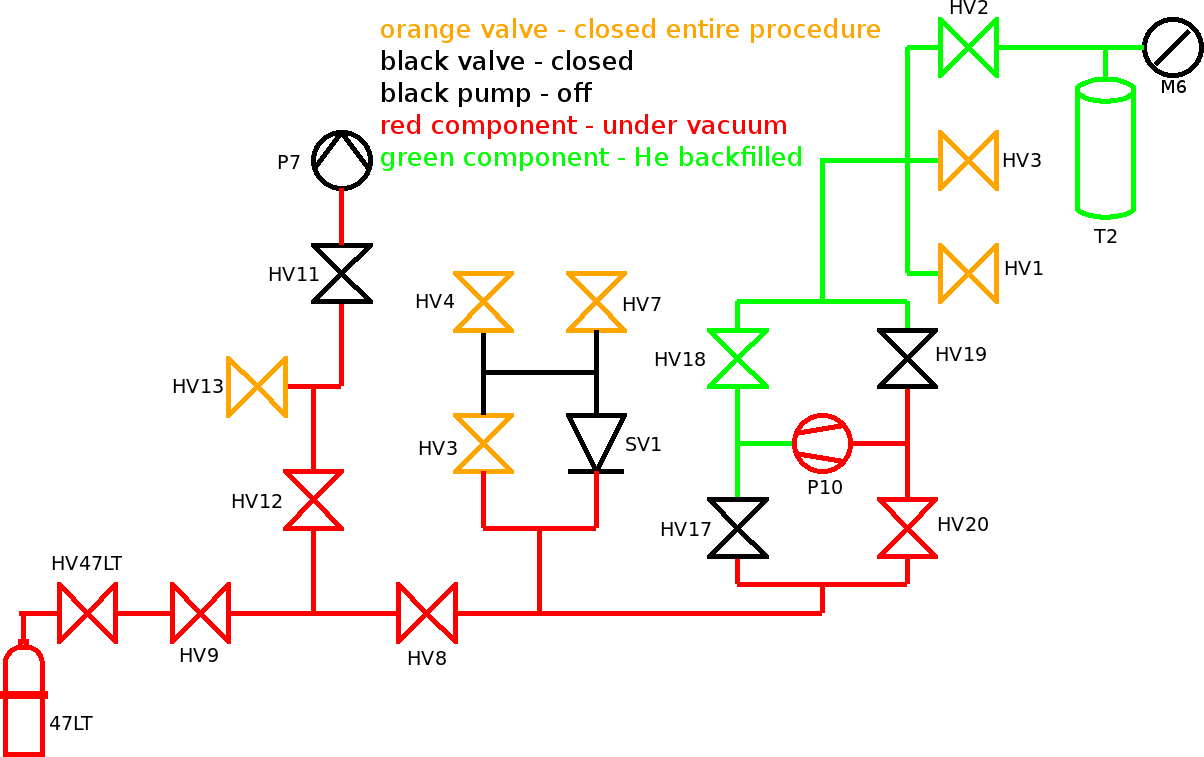
\includegraphics[width=\textwidth]{./he-3-transfer-08-open-hv20.png}
 % he-3-transfer-08-open-hv20.png: 0x0 pixel, 0dpi, 0.00x0.00 cm, bb=
 \caption{Open HV20 to pump gas out of pressurized cylinder and the rest of the system into T2.}
 \label{f}
\end{figure}

\begin{figure}[htbp!]
 \centering
 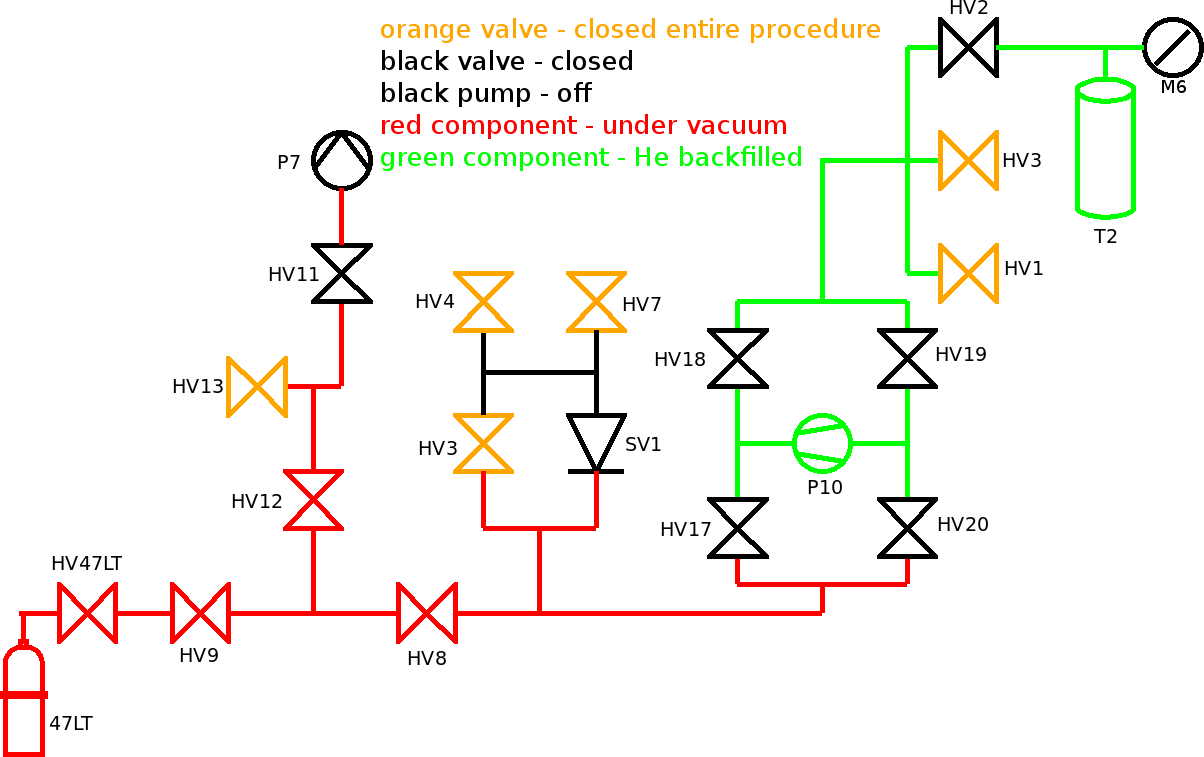
\includegraphics[width=\textwidth]{./he-3-transfer-09-turn-off-p10.png}
 % he-3-transfer-09-turn-off-p10.png: 0x0 pixel, 0dpi, 0.00x0.00 cm, bb=
 \caption{Isolate P10 and the $^3$He tanks from the rest of the system.}
 \label{g}
\end{figure}

\end{document}
